% Parler ici de la hiérarchie de classes et des structures de données, de git, de github, et de Doxygen, licence GPL
\subsection{Organisation du travail.}
  Nous avons utilisé \emph{git}, couplé à un dépôt \emph{git} sur \emph{github}, qui affiche de jolis graphes de la progression du projet, 
  et a un système d'\emph{issues}, ce qui permet d'assigner des objectifs avec une date. 
   La création de branches a permis de mener efficacement un travail parallèle, et l'outil de résolution des conflits \emph{meld} a grandement contribué à ce que les moments
  de fusion de branches soient extrêmement rapides.
  Le dépôt étant public, il a fallu mettre une licence adaptée : la licence \emph{GPL}.
  
  Le code est commentée avec des commentaires \emph{Doxygen}, ce qui permet de générer automatiquement une documentation au format html.
  
\subsection{Organisation du projet.}

\paragraph{Hiérarchie de classe : } 
Les différentes abstractions qui permettent de rendre une scène ont été conçues pour être les plus génériques possibles. Dans la mesure du possible, les différents  objets insérables dans une scène sont une classe abstraite pure : \verb|Solid|, \verb|Light|...
\begin{figure}[h]
\begin{center}
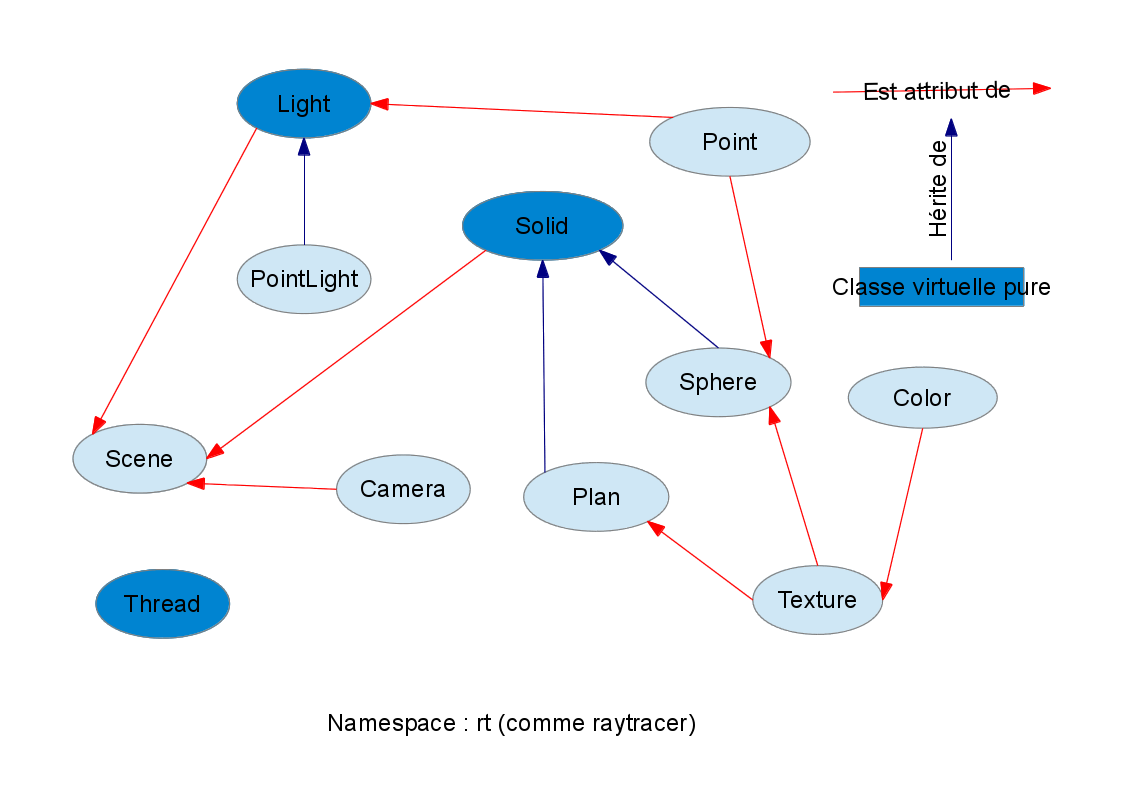
\includegraphics[scale=0.35]{hierarchie.png}
\end{center}
\caption{Hiérarchie de classes.}
\end{figure}

Ainsi, pour créer un nouveau type d'objet, par exemple, une sphère, il faut hériter de \verb|Solid| puis implémenter les quatre méthodes virtuelles 
pures de \verb|Solid| suivantes :

\begin{lstlisting}
virtual bool intersect(const Point& pos, const vector& vect) const = 0;

virtual Point getIntersection(const Point& point, const vector& vect) const = 0;

virtual Point autreCote(const Point& point, const vector& vect,	const Point& act) const = 0;

virtual vector getNormal(const Point& p, const vector& v) const = 0;
\end{lstlisting}

Pour créer un nouveau type de lampe, comme une lumière ponctuelle, il faudra hériter de \verb|Light|, et implémenter :
\begin{lstlisting}
virtual color illuminate(const Point& point, const Solid* m, const vector vision) const = 0;
\end{lstlisting}

Toutes les classes du lanceur de rayons sont placées dans l'espace de nom \emph{rt}. Pour créer une scène particulière, il est
conseillé de créer une classe \emph{MyScene} qui dérive de \emph{Scene}, ce qui permet de gérer les allocations et désallocations 
mémoire des objets dans la scène proprement. Ces classes, qui sont du ressort de l'utilisateur, ne se trouvent donc pas dans l'espace
 de nom \emph{rt}.

\paragraph{Structures de données : }
Les structures de données utilisées pour conserver les objets dans une scène (lampes, solides), sont des \verb|vector| : 
\begin{lstlisting}
std::vector<Solid*> objets;
std::vector<Light*> lights;
\end{lstlisting}
Les \emph{vector} ont l'inconvénient d'occasionner un temps de recherche linéaire de l'intersection entre les objets dans la scène et un rayon lancé. 
Des structures de données plus efficaces mais plus complexes, \emph{octree} et \emph{voxels}, existent.